\documentclass{beamer}

\usetheme[numbering=none, progressbar=frametitle]{metropolis}
\usepackage{graphicx} % Allows including images
\usepackage{booktabs} % Allows the use of \toprule, \midrule and \bottomrule in tables
\usepackage{tikz}
\usepackage{siunitx}
\usepackage{amsmath}

\title{MCMD: Time evolution of stellar clusters}
\author{Alex Arash Sand Kalaee}
\institute{Division of Mathematical Physics, Lund University}
\date{Wednesday, June 5, 2019}
\begin{document}
\maketitle

\begin{frame}
\frametitle{Objective}
Given a cluster of a million stars, what is the likely time evolution of the
population of main sequence stars and remnants, cluster mass
and the mass/luminosity ratio over a period of 15 Gyr?
\end{frame}

\begin{frame}
\frametitle{Distribution of stellar mass}
We are provided the distribution
\begin{equation*}
f(m) = m^{-\gamma}
\end{equation*}
with $\gamma = 1.3$ for $0.08 < m < 0.5$, $\gamma=2.2$ for $0.5 < m < 1$ and
$\gamma = 2.7$ for $1 < m < 120$.

We use importance sampling with $g(m) = m^{-2.2} \geq f(m)$ and can now
sample random stellar clusters.

We will sample the statistics from 10,000 iterations of the cluster.
\end{frame}
\begin{frame}
\frametitle{Distribution of stellar mass}
\begin{center}
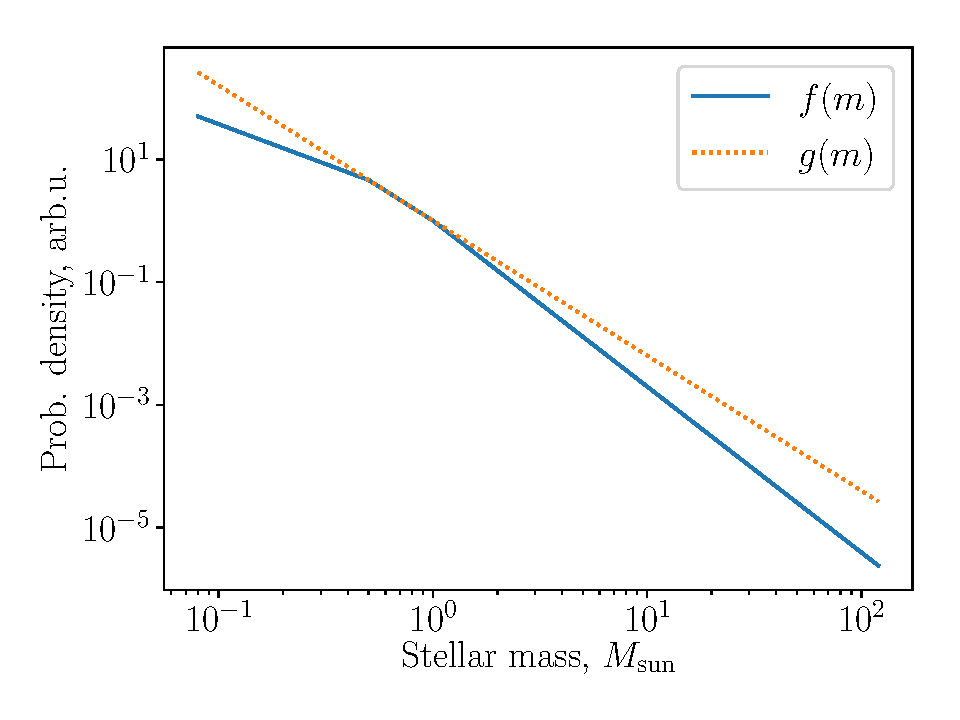
\includegraphics[width=0.9\textwidth]{dist.pdf}
\end{center}
\end{frame}

\begin{frame}
\frametitle{Stellar lifetimes}
The lifetime of a main sequence star is
\begin{equation*}
\tau = 10^{10}\left(\frac{m}{M_\mathrm{sun}}\right)^{-2.5}\mathrm{ yr}
\end{equation*}
We assume that the masses are constant during the lifetimes of the stars.
\end{frame}

\begin{frame}
\frametitle{Remnants}
Depending on the mass of the star it can become one of three types of
remnants

\begin{tabular}{c|ccc}
Type & Mass & Star mass& Creation time, yr.\\
\hline
White dwarf & 0.6 & 0.08 -- 8 & $5.5\cdot10^{7}$ -- $5.5\cdot10^{12}$\\
Neutron star & 1.4 & 8 -- 30 & $2.0\cdot10^{6}$ -- $5.5\cdot10^{7\phantom{0}}$ \\
Black hole & 10 & 30 -- 120 & $6.3\cdot10^{4}$ -- $2.0\cdot10^{6\phantom{0}}$
\end{tabular}

Remnants have zero luminosity!
\end{frame}

\begin{frame}
\frametitle{Time evolution -- population}
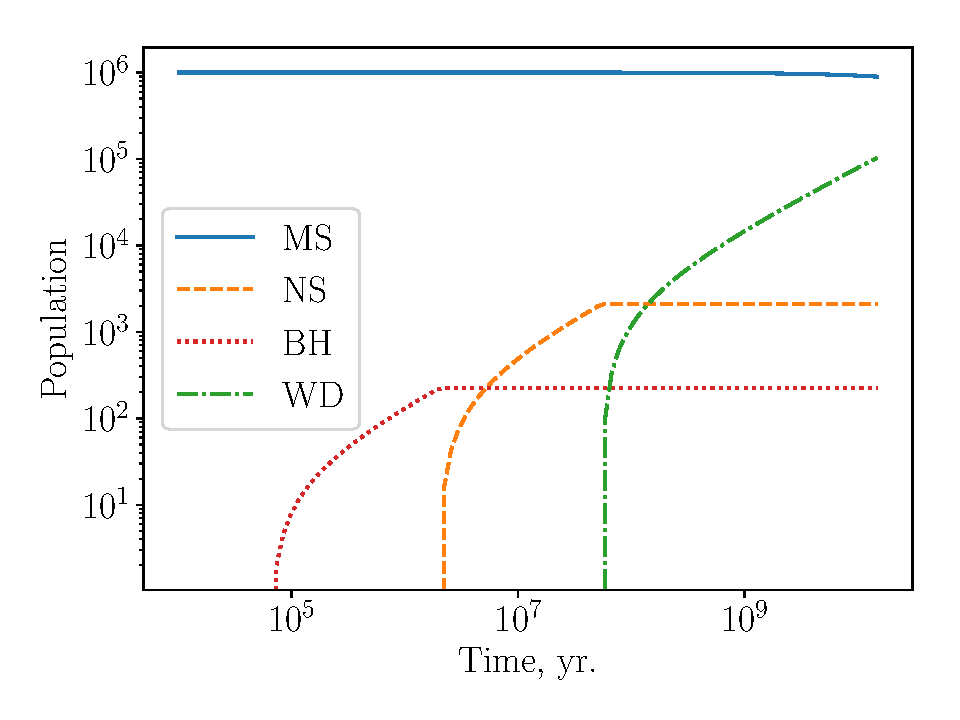
\includegraphics[width=0.8\textwidth]{remn.pdf}
\end{frame}

\begin{frame}
\frametitle{Time evolution -- mass}
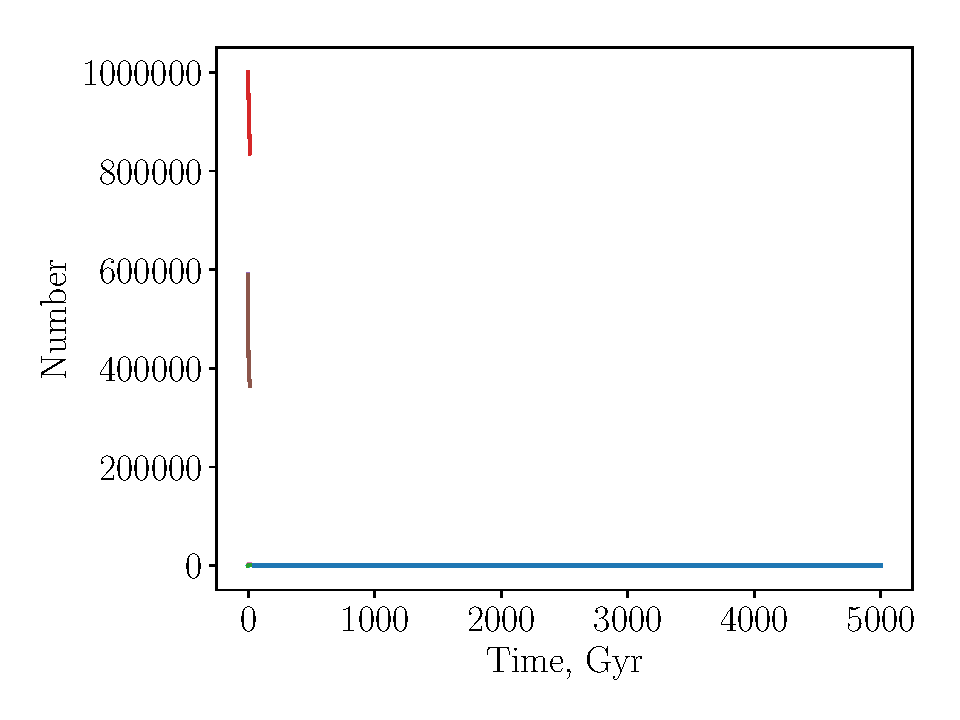
\includegraphics[width=0.8\textwidth]{sm.pdf}
\end{frame}

\begin{frame}
\frametitle{Luminosity}
From a very rough model we assume that luminosity and mass are constant
during the lifetime of the star and their ratio is related to the lifetime
\begin{equation*}
\tau\propto \frac{m}{L}
\end{equation*}

Hence, in some appropriate system of units,
\begin{equation*}
L = \frac{m}{\tau}
\end{equation*}
\end{frame}

\begin{frame}
\frametitle{Time evolution -- mass-luminosity ratio}
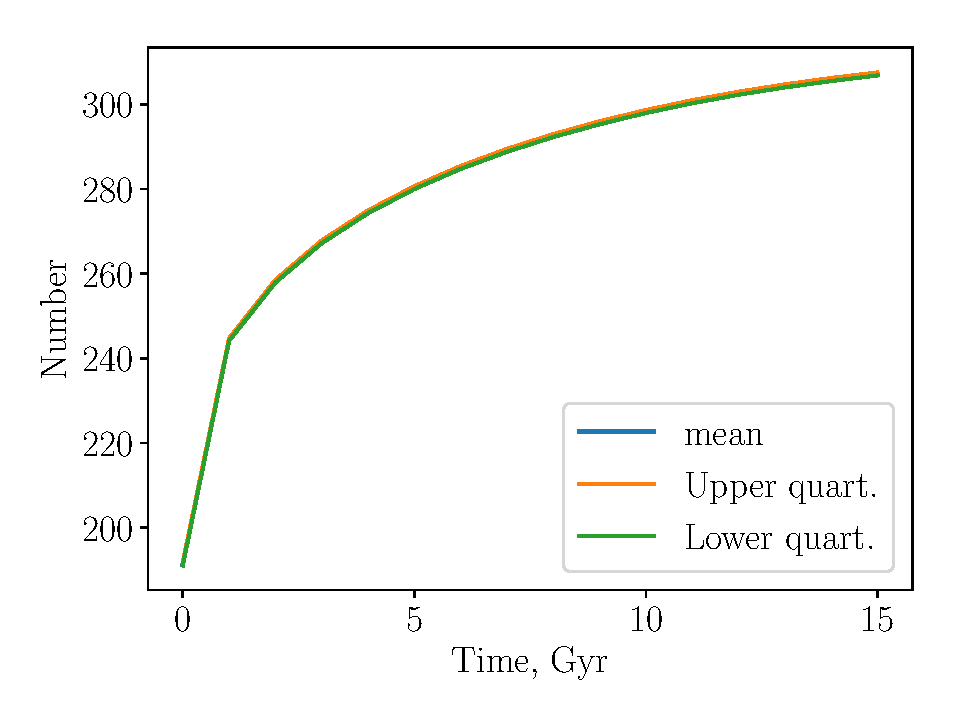
\includegraphics[width=0.8\textwidth]{lm.pdf}

Surviving stars have a large lifetime, hence larger $m/L$-ratio!
\end{frame}



\begin{frame}
\frametitle{State after 12 Gyr}
After 12 Gyr the average population is

\begin{tabular}{c|cccc}
Type & MS stars & White dwarfs & Neutron stars & Black holes\\
\hline
Number & 908772 & 88896 & 2107 & 225
\end{tabular}
\end{frame}

\end{document}
